\documentclass[a4paper,11pt,spanish]{article}

\textwidth 18.5cm
\textheight 26cm
\topmargin -2cm
\oddsidemargin -1.5cm
\parskip .3em
\parindent 0cm

%your favourite packages here
\usepackage[spanish]{babel}
% \usepackage{lineno}
% \usepackage{mathptmx}
%\usepackage{sublabel}
%\usepackage{psfrag,graphicx}
%\usepackage{subfigure}
\usepackage{amsmath}
\usepackage{amssymb}
\usepackage{amsfonts}
\usepackage{bm}
%\usepackage{bbm}
\usepackage{color}
%\usepackage{overpic}
\usepackage{latexsym}
\usepackage{epstopdf}
\usepackage{color}
%\usepackage{times}
%\usepackage{stmaryrd}

\usepackage{psfrag,graphicx}
%\usepackage{picins}
%\usepackage{epsf}
\usepackage{natbib}
\usepackage{epstopdf}\DeclareGraphicsRule{.tif}{png}{.png}{`convert #1 `basename
#1 .tif`.png}
%\usepackage{appendix}
%\usepackage{dsfont}
%\usepackage{mathtools}

\definecolor{mygrey}{gray}{0.35}
\definecolor{myblue}{rgb}{0.2,0.2,0.8}
\definecolor{myzard}{cmyk}{0,0,0.05,0}
\definecolor{mywhite}{rgb}{1,1,1}
\definecolor{myred}{rgb}{1,0.,0.3}

\def \barl {\begin{array}{rl}}
\def \ea {\end{array}}
%\definecolor{myblue}{named}{MidnightBlue}
\usepackage{hyperref}
\def\beq{\begin{equation}}
\def\eeq{\end{equation}}
\def\ba{\begin{align}}
\def\enda{\end{align}}
\def\bi{\begin{itemize}}
\def\ei{\end{itemize}}
\def\bs#1{\boldsymbol{#1}}
\def\txt#1{\textrm{#1}}

\newcommand{\eq}[1]{Eq.\;(\ref{#1})}

\newcommand{\sgn}{\operatorname{sgn}}
\def\C{{\mathbb{C}}} \def\F{{\mathbb{F}}}
\def\N{{\mathbb{N}}} \def\Q{{\mathbb{Q}}}
\def\R{{\mathbb{R}}} \def\Z{{\mathbb{Z}}}
\def\cH{{\mathcal H}}
\def\bfsigma{\boldsymbol{\sigma}}
\def\bfmu{\boldsymbol{\mu}}
\def\dd{\mathord{\rm d}} \def\Det{\mathop{\rm Det}}
\def\dist{\mathop{\rm dist}} \def\ee{\mathord{\rm e}}
\def\End{\mathord{\rm End}} \def\ev{\mathord{\rm ev}}
\def\id{\mathord{\rm id}} \def\ii{\mathord{\rm i}}
\def\min{\mathord{\rm min}} \def\mod{\mathord{\rm mod}}
\def\prob{\mathord{\rm prob}}
\def\tr{\mathop{\rm Tr}}
\def\half{\textstyle\frac{1}{2}}
\def\third{\textstyle\frac{1}{3}}
\def\fourth{\textstyle\frac{1}{4}}

\graphicspath{{figs/}}

\newcommand{\da}{\downarrow}
\newcommand{\ua}{\uparrow}

\renewcommand{\ii}{{\rm i}}
\renewcommand{\ee}{{\rm e}}

%brackets
 \newcommand{\ket}[1]{|#1\rangle}
 \newcommand{\bra}[1]{\langle #1|}
 \newcommand{\braket}[2]{\langle #1|#2\rangle}

 \newcommand{\ketbra}[2]{\ket{#1}\bra{#2}}
 \newcommand{\proj}[1]{\ketbra {#1}{#1}}
 \newcommand{\biket}[2]{\ket{#1\;#2}}
 \newcommand{\bibra}[2]{\bra{#1\;#2}}
 %\newcommand{\ketbradif}[2]{\biket {#1}{#2}\bibra {#1}{#2}}
% \newcommand{\preespacio}{\!\text{\hspace{0.2 ex}}}
% \newcommand{\postespacio}{\!\text{\hspace{0.75 ex}}}


% \graphicspath{{Plots/}}

\begin{document}

%\title[Short Title]{Ejercicios para el curso de Introducci\'on a la \'Optica Cu\'antica}

\author{C. Cormick}

% \maketitle

\noindent{\large \bf Procesamiento Cu\'antico de la Informaci\'on - C. Cormick, FING - 1er sem. 2025}\\

\noindent{\large \bf Práctico 2 - ABC de información cuántica}\\

\vspace{5pt}

\noindent Aclaraci\'on: Muchos de estos ejercicios fueron tomados de o inspirados en ``Virginia Tech Quantum Information Science and Engineering Summer School 2022'' por Sophia E. Economou, Edwin Barnes, y Jamie Sikora.

\bigskip

\begin{enumerate}

    \item {\bf No clonaci\'on.} En este ejercicio vemos por qu\'e las reglas de la cu\'antica no permiten ``clonar'' (o copiar) estados cu\'anticos arbitrarios desconocidos (un paper de 1982, aunque el resultado había sido ya probado antes... más info en su Wikipedia amiga). 
    
    Supongamos que tenemos una m\'aquina que copia los estados ``cl\'asicos'' de un qubit de entrada a un qubit auxiliar ``target'' preparado en blanco, como indica la siguiente figura:
    
    \begin{center}
     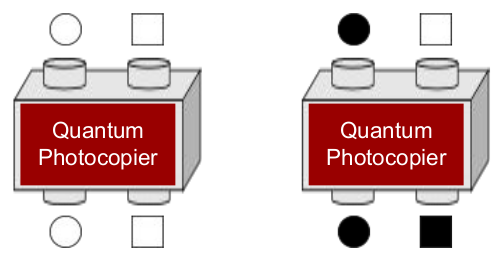
\includegraphics[width=170pt]{no-cloning.png}
    \end{center}

    Mostrar que si el qubit de entrada que se desea copiar se encuentra en un estado neblinoso que combina blanco y negro, el resultado a la salida {\bf no} son dos qubits en ese mismo estado (como deber\'ia hacer una fotocopiadora de qubits) sino un estado entrelazado de ambos.
    \medskip
    
    \item {\bf Algoritmo de Deutsch}. Este es un algoritmo simple propuesto en 1985. Nuestra premisa es la siguiente: tenemos un juego en el que hay dos puertas y un bot\'on que puede abrir ambas a la vez, pero no una sola. Detr\'as de alguna de las dos puertas hay un mont\'on de plata, pero podr\'ia ser que detr\'as de una de ellas (solo una) haya un tigre que no quisi\'eramos liberar al abrir las puertas. Idealmente, queremos obtener el dinero, pero solo si tenemos la seguridad de que no hay tigre... si lo hay preferimos escapar pobres y con vida.
    
    El juego incluye una compuerta ``or\'aculo'' que nos permite averiguar si detr\'as de una dada puerta hay o no un tigre. M\'as precisamente, las dos puertas est\'an identificadas con un cuadrado blanco y uno negro respectivamente. La compuerta or\'aculo es una compuerta de dos qubits: el primero, representado por un c\'irculo, es el target y el segundo, representado por un cuadrado, identifica sobre qu\'e puerta queremos consultar. La compuerta or\'aculo aplica un NOT sobre el qubit target si y s\'olo si detr\'as de la puerta correspondiente al segundo qubit efectivamente hay un tigre. Las reglas se representan a continuaci\'on:
    
    \begin{center}
     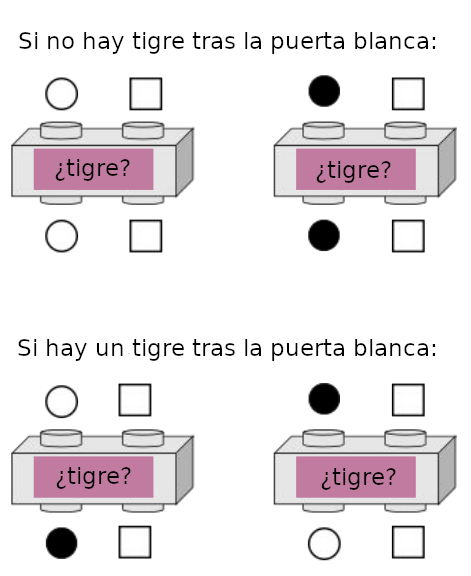
\includegraphics[width=153pt]{gate_white_door.png}\hspace{70pt}
     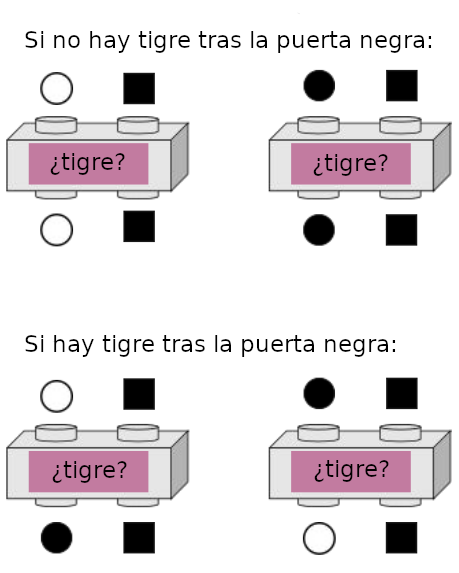
\includegraphics[width=150pt]{gate_black_door.png}
    \end{center}

    Notar que el qubit cuadrado indica la puerta sobre la que se obtiene informaci\'on, mientras que el qubit circular cambia de color si tras la puerta en cuestión hay un tigre. Notar tambi\'en que si solo podemos usar bits cl\'asicos, o qubits en estados cl\'asicos, entonces para saber con seguridad si hay o no un tigre en alguna parte tenemos que usar el or\'aculo dos veces; no es posible usarlo solo una vez y llevarse el dinero sin arriesgarse. Pero las reglas del juego nos permiten usar el or\'aculo {\it una \'unica vez}. A continuaci\'on veremos c\'omo hacerlo usando la cu\'antica:
    
    \begin{enumerate}
     \item Mostrar c\'omo crear el estado neblinoso de la figura (notar que es un estado separable, es decir solo hacen falta compuertas de un qubit):
     \begin{center}
      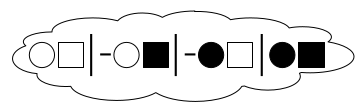
\includegraphics[width=140pt]{Deutsch_1.png}
     \end{center}
     
     \item Calcular cu\'al es la salida de la compuerta or\'aculo si el estado de entrada es el del \'item anterior, en cada uno de los tres casos de inter\'es, es decir: i) si no hay ning\'un tigre, ii) si hay tigre detr\'as de la puerta blanca, o iii) si lo hay detr\'as de la puerta negra.

     \item Ver cu\'al es el estado que se obtiene en cada uno de esos tres casos si luego de la compuerta or\'aculo se aplica una compuerta de Hadamard a cada qubit.
     
     \item Notar que juntando estos pasos podemos averiguar si hay o no hay tigre en un \'unico paso (dando por v\'alida la promesa de que solo puede haber un tigre y no dos). Ver que la clave de este algoritmo es la utilizaci\'on de un autoestado de la compuerta NOT en el qubit circular; esto me ``devuelve'' un signo sobre el estado del qubit cuadrado en forma tal que el estado final del cuadrado depende solo de si hay un tigre, pero no de en qu\'e puerta est\'a.
     
     \item Opcional: ver que con este algoritmo no podemos distinguir entre un caso sin tigres y uno con dos tigres, y por eso la promesa es importante.
     
     \item Programar todo esto en el simulador IBM; notar que parte de la tarea es programar el or\'aculo, que va a ser diferente en cada uno de los tres casos.
    \end{enumerate}
    \medskip

    \item {\bf Estados de Bell}
    
    \begin{enumerate}
     \item Dise\~nar un circuito que obedezca las siguientes reglas de entrada-salida:
    
    \begin{center}
     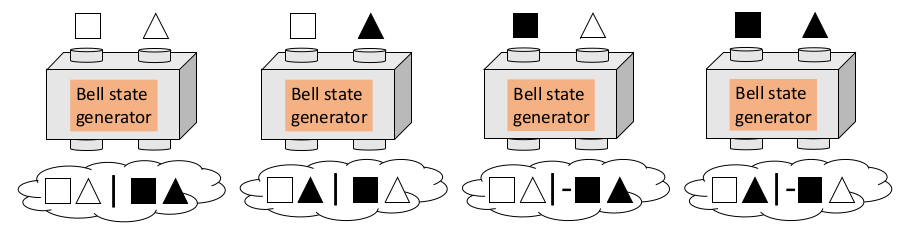
\includegraphics[width=0.7\textwidth]{Bell_state_generator.png}
    \end{center}
    
    \item Verificar que, dado uno de esos estados, si se realiza una medici\'on de ambos qubits no hay modo de distinguir en forma perfecta de cu\'al de los cuatro estados se trataba, mientras que si se hace una medici\'on sobre un \'unico qubit ambos resultados (blanco o negro) son equiprobables en los cuatro casos.
    
    \item Dise\~nar un circuito que permita distinguir entre los cuatro estados de Bell, es decir, el circuito debe ser tal que si el estado de entrada es uno de los cuatro estados de Bell, luego de pasar por el circuito puedo medir los dos qubits y distinguir de cu\'al de los cuatro estados se trataba.
    
    \item Qu\'e pasa si concateno el circuito generador de estados de Bell con el circuito que distingue estados de Bell? Ver c\'omo se puede simplificar la secuencia de compuertas.

    \item Probar los ejercicios anteriores en el simulador IBM.
    \end{enumerate}
    \medskip
    
    \item {\bf Transformaci\'on de estados de Bell.} Ver c\'omo cambia cada estado de Bell si se aplica sobre el primer qubit una de las siguientes compuertas: 
    
    \begin{enumerate}
     \item Z
     \item X
     \item Z y luego X (o al rev\'es)
    \end{enumerate}

    (Estas transformaciones son la base del protocolo de ``superdense coding'' - publicado en 1992).
    
    Ver tambi\'en c\'omo cambia el resultado si estas compuertas se aplican sobre el segundo qubit en lugar del primero. Probar estas transformaciones con el simulador IBM (en combinaci\'on con los circuitos de generaci\'on y medici\'on de estados de Bell dise\~nados en el problema anterior).
    
    \item {\bf Teleportaci\'on.} En este protocolo (propuesto en 1993) se quiere enviar {\it el estado desconocido} de un qubit a un laboratorio distante. El estado desconocido lo representamos con el s\'imbolo $\Psi$. Los laboratorios comparten un par de qubits entrelazados, en el primero de los estados de Bell del ejercicio 3. Entre los laboratorios pueden enviarse informaci\'on cl\'asica, pero no qubits. (Notar que si el estado $\Psi$ fuera conocido, o si se lo pudiera medir sin alterarlo, bastar\'ia con enviar la informaci\'on necesaria para prepararlo.) El esquema de teleportaci\'on se muestra en la figura:
    
    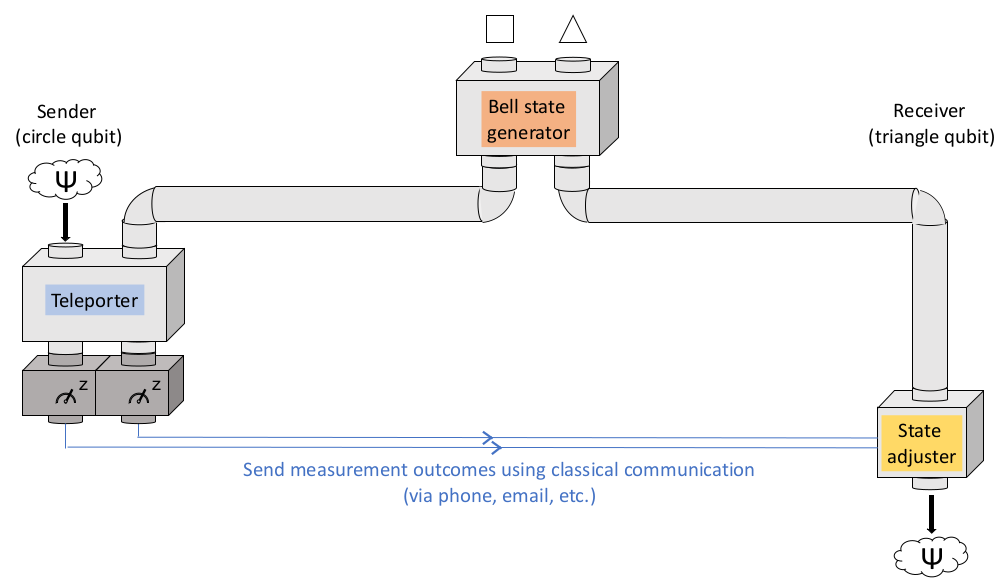
\includegraphics[width=0.8\textwidth]{teleportation.png}
    
    \begin{enumerate}
     \item Las reglas de entrada-salida de la ``caja teleportadora'' est\'an dadas por el siguiente esquema:
     
     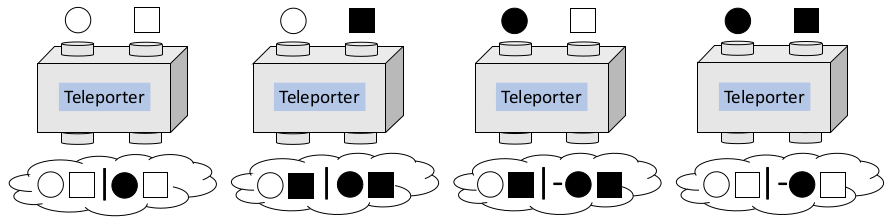
\includegraphics[width=0.7\textwidth]{teleporter_box.png}
     
     Dise\~nar un circuito que cumpla con estas reglas. Verificar que este mismo circuito se puede usar como medidor de estados de Bell (o sea puede ser la soluci\'on del problema 3c).
     
     \item Luego de que se realice la medici\'on sobre los primeros dos qubits, el qubit ``target'' queda desentrelazado, pero su estado depende no solo de $\Psi$ sino tambi\'en del resultado de las mediciones. Esos resultados se env\'ian por un canal cl\'asico y en el segundo labo se aplican compuertas de correcci\'on para recuperar el estado $\Psi$.
%     \begin{itemize}
%      \item 00: sin correcci\'on
%      \item 01: X
%      \item 10: Z
%      \item 11: XZ
%     \end{itemize}
    Considerar el caso de que $\Psi$ sea uno de los siguientes estados:
    \begin{center}
    
\includegraphics[width=130pt]{examples.png}
    \end{center}
    
    Calculando el estado de los tres qubits en cada paso del protocolo, ver qu\'e correcciones hay que hacer en cada caso para obtener el resultado final correcto.
    
    \item Verificar que si se combinan las correcciones correspondientes a los dos ejemplos se obtiene un conjunto de cuatro correcciones diferentes que sirve para los dos casos (es decir, las correcciones obtenidas de un caso no arruinan el estado si resulta ser el otro). Recordar para esto que un signo menos global no cambia el estado.
    
    \item Programar el circuito completo en el simulador IBM (incluyendo las correcciones condicionales a los resultados) y verificar que anda bien para los siguientes posibles estados iniciales:
    \begin{center}
    
\includegraphics[width=200pt]{more_examples.png}
    \end{center}
    (Estos son los \'unicos estados de un qubit que conocemos por ahora, pero este mismo circuito de teleportaci\'on funciona para estados arbitrarios, como veremos m\'as adelante).
    
    \end{enumerate}
    
%    \newpage

    \item {\bf Correcci\'on cu\'antica de errores}. Programar en el simulador IBM un código de corrección de errores tipo bit-flip y uno tipo phase-flip, incluyendo las operaciones de medición y corrección. Verificar su correcto funcionamiento introduciendo los errores correspondientes en cualquiera de los qubits. Ver qué pasa si hay errores en más de un qubit.
    
    \medskip
    
    \item {\bf N\'umeros complejos.} (Repaso para quien lo necesite.)
 \begin{enumerate}
  \item Calcular el producto de $4\,e^{\rm i\pi}$ por $0,2\,e^{-\rm i\pi/4}$ expl\'icitamente usando m\'odulo y fase. Graficar en el plano complejo ambos factores y su producto. Luego escribir cada uno de esos n\'umeros en la forma $x+{\rm i}y$, multiplicar nuevamente, y verificar que el resultado coincide con el obtenido anteriormente.

  \item Considerar los siguientes n\'umeros complejos: $z_1=1+5i$, $z_2=2-i$. Dibujar en el plano complejo, calcular el m\'odulo $|z_j|$ de cada n\'umero y estimar, a ojo a partir del dibujo, el valor del \'angulo $\varphi_j$ tal que $z_j = |z_j|e^{i\varphi_j}=|z_j|(\cos\varphi_j + {\rm i}\sin\varphi_j)$.

  \item Multiplicar $z_1$ por $z_2$ y representar el n\'umero resultante en el plano complejo.

  \item Calcular el m\'odulo del resultado, y verificar que es igual al producto $|z_1|\times |z_2|$. Estimar a ojo el \'angulo $\varphi$ del resultado y verificar que es parecido a la suma $\varphi_1+\varphi_2$.

  \end{enumerate}
  \smallskip

%  \item {\bf Estados neblinosos con coeficientes no uniformes.} Es posible crear estados con coeficientes diferentes partiendo de otros estados donde todos los t\'erminos no nulos tienen iguales coeficientes. Por ejemplo, tomar el siguiente estado:

%  \begin{center}
%   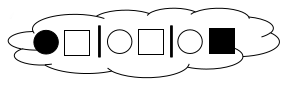
\includegraphics[width=120pt]{neblinoso_3.png}
%  \end{center}

%  Mostrar que si se aplica una compuerta $H$ al primer qubit, el estado resultante tiene algunos t\'erminos repetidos (pero no todos).
%  \smallskip

  \item {\bf Probabilidades en estados con coeficientes arbitrarios.} Consideramos los siguientes estados de 1 qubit m\'as generales, que contienen t\'erminos repetidos:

  \begin{center}
   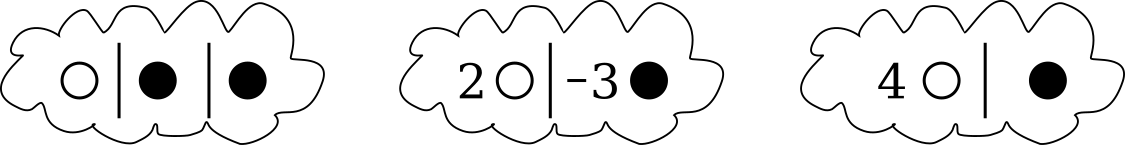
\includegraphics[width=250pt]{coeficientes.png}
  \end{center}

  \begin{enumerate}
   \item Calcular en cada caso la probabilidad de hallar el qubit blanco al realizar una medici\'on.

   \item Expresar los estados del problema anterior con coeficientes normalizados.
  \end{enumerate}
  \smallskip

  \item {\bf Mediciones completas y parciales.} Considerar ahora los siguientes estados de dos qubits:

  \hspace{-20pt} 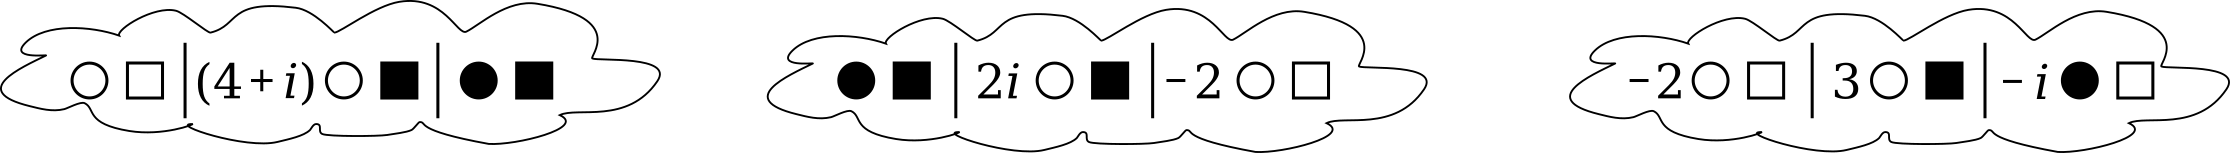
\includegraphics[width=480pt]{coeficientes_2qubits.png}

  \begin{enumerate}
   \item Expresar cada estado con coeficientes normalizados. Indicar los resultados posibles al realizar una medici\'on sobre los dos qubits, y sus correspondientes probabilidades.

   \item A partir del \'item anterior, calcular la probabilidad de obtener como resultado ``blanco'' al medir el primer qubit. Explicar qu\'e regla debe usarse para calcular dichas probabilidades directamente a partir de los coeficientes del estado neblinoso.

   \item Para cada uno de los estados considerados, explicar cu\'al es el estado final del sistema si al medir el primer qubit se obtiene ``blanco'' y cu\'al si se obtiene ``negro''. Expresar los estados resultantes con coeficientes normalizados.
  \end{enumerate}
  \smallskip

  \item {\bf Entrelazamiento.} Considerando el estado neblinoso m\'as general de dos qubits, hallar qu\'e condiciones deben cumplir los coeficientes $a, b, c, d \in \mathbb{C}$ para que el estado sea separable (no entrelazado):

  \begin{center}
   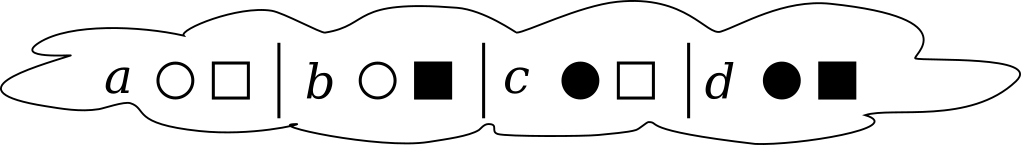
\includegraphics[width=250pt]{entrelazamiento.png}
  \end{center}

  \smallskip

    \item {\bf OPCIONAL: ``Paradoja'' de Mermin.} Este ejercicio est\'a tomado de ``Quantum mysteries revisited'' (1990) y es un poco largo, hay que tomarlo con calma. Vale resolver el primer \'item ayud\'andose por el paper de Mermin, y vale volver sobre el segundo \'item m\'as adelante en la materia (algunas cosas se har\'an m\'as f\'aciles de resolver, aunque no necesariamente de entender). \textexclamdown El segundo \'item no se puede resolver copi\'andose del paper de Mermin! Hay algunos detalles cambiados.

    Consideremos tres detectores con interruptores que pueden cambiarse libremente entre las posiciones 1 o 2, y que reciben tres part\'iculas preparadas de alguna manera conjunta en una misma fuente. Luego de recibir las part\'iculas, cada detector puede emitir una luz naranja o azul que puede depender de la posici\'on del interruptor y del estado de la part\'icula recibida.

    Se pide cumplir con las siguientes condiciones:
    \begin{itemize}
     \item Si un \'unico detector est\'a en 1, entonces debe verse un n\'umero impar de luces naranjas.
     \item Si los tres detectores est\'an en 1, entonces debe verse un n\'umero par de luces naranjas.
    \end{itemize}
    (El caso en que hay un n\'umero par de detectores en 1 no nos interesa).

    \begin{enumerate}
     \item Mostrar que no hay ninguna elecci\'on cl\'asica de ``instrucciones'' que las part\'iculas puedan llevar que cumpla con estos requisitos si los tres detectores est\'an en tres regiones incomunicadas entre s\'i y las posiciones de los interruptores son desconocidas fuera de sus correspondientes ubicaciones.
    \end{enumerate}

    \begin{minipage}{280pt}
     \begin{enumerate}
      \item[(b)] Por esta vez, vamos a tener un estado cu\'antico tan largo que nos conviene escribir las distintas componentes superpuestas apiladas en vez de una al lado de la otra. Mostrar que el estado de la figura cumple los requisitos del desaf\'io de Mermin, suponiendo que:
     \begin{itemize}
      \item Cuando un interruptor est\'a en 1, se aplica sobre la correspondiente part\'icula una compuerta de Hadamard antes de medir, mientras que si est\'a en 2 se mide directamente.
      \item Si se observa un qubit blanco se emite una luz naranja, mientras que para un qubit negro se emite una luz azul.
     \end{itemize}

     \item[(c)] Mostrar que el ``estado de Mermin'' de la figura se puede crear a partir del estado inicial con los tres qubits blancos aplicando tres compuertas de Hadamard seguidas por compuertas C-Z.

     \item[(d)] Usando el \'item anterior, verificar en el simulador IBM que el estado efectivamente cumple las condiciones de Mermin. Probar con todas las elecciones posibles de los interruptores que sean relevantes para el problema.

%    \item Verificar la siguiente afirmaci\'on que por ahora ser\'a misteriosa: el ``estado de Mermin'' de la figura queda exactamente igual si se aplican sobre \'el las siguientes compuertas:
%    \begin{enumerate}
%     \item X sobre el primer qubit y Z sobre los otros dos.
%     \item X sobre el segundo qubit y Z sobre los otros dos.
%     \item X sobre el tercer qubit y Z sobre los otros dos.
%     \item Si se aplica X sobre los tres qubits a la vez, el estado queda igual pero aparece un signo - global.
%    \end{enumerate}

    \end{enumerate}

    \end{minipage}\hspace{30pt}
%
    \begin{minipage}{140pt}
    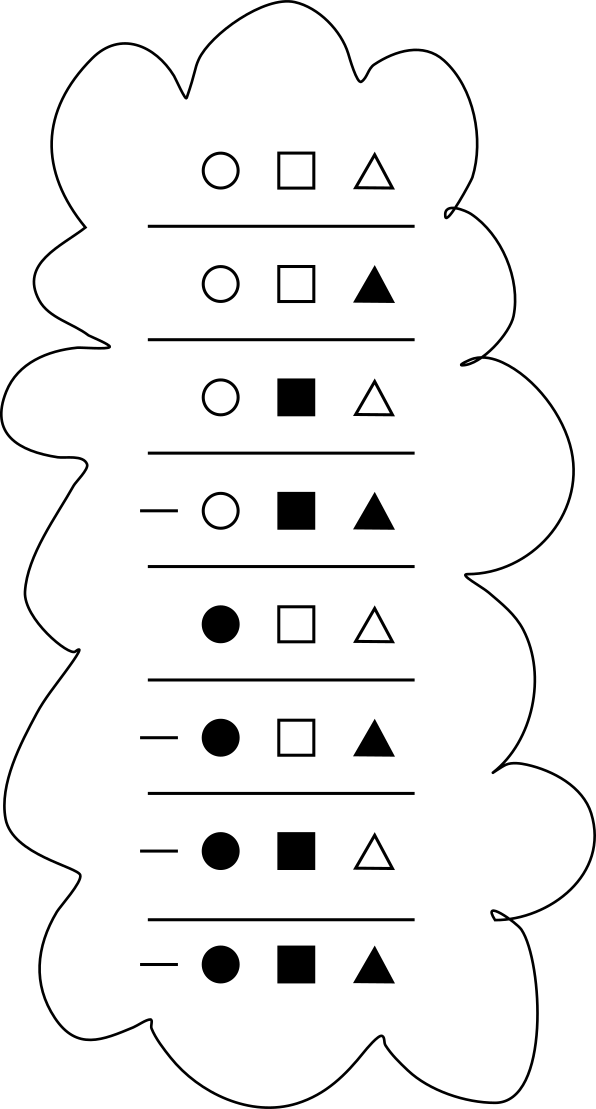
\includegraphics[width=140pt]{Mermin.png}
    \end{minipage}


\end{enumerate}


\end{document}
